\documentclass[tikz,border=10pt]{standalone}
\usepackage{tikz}
\usetikzlibrary{calc}

\begin{document}
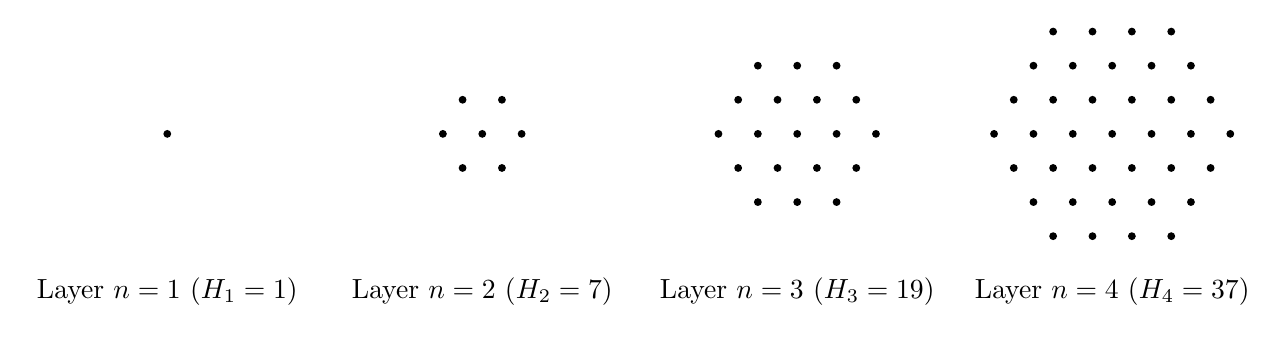
\begin{tikzpicture}[dot/.style={circle, fill=black, inner sep=1pt}]

% Controls
\def\hexstep{0.5}
\def\xgap{6}

% n=1 → just center
% n=2 → center + 1 ring
% n=3 → center + 2 rings, etc.
\newcommand{\drawHexagonDots}[3]{%
  \begin{scope}[shift={(#2,#3)}]
    \node[dot] at (0,0) {}; % center dot always

    \pgfmathtruncatemacro{\rings}{#1 - 1}
    \ifnum\rings>0
      \foreach \r in {1,...,\rings} {
        \pgfmathsetmacro{\rad}{\r * \hexstep}
        \foreach \side in {0,...,5} {
          \pgfmathsetmacro{\angleA}{60*\side}
          \pgfmathsetmacro{\angleB}{60*(\side+1)}
          \coordinate (A) at (\angleA:\rad);
          \coordinate (B) at (\angleB:\rad);
          \foreach \k in {0,...,\numexpr\r-1} {
            \pgfmathsetmacro{\t}{\k/\r}
            \path ($(A)!{\t}!(B)$) node[dot] {};
          }
        }
      }
    \fi
  \end{scope}
}

% Draw H₁ through H₄
\drawHexagonDots{1}{-6}{0}  % H₁ = 1
\drawHexagonDots{2}{-2}{0}  % H₂ = 7
\drawHexagonDots{3}{ 2}{0}  % H₃ = 19
\drawHexagonDots{4}{ 6}{0}  % H₄ = 37

% Labels
\node at (-6,-2) {Layer $n=1$ ($H_1 = 1$)};
\node at (-2,-2) {Layer $n=2$ ($H_2 = 7$)};
\node at ( 2,-2) {Layer $n=3$ ($H_3 = 19$)};
\node at ( 6,-2) {Layer $n=4$ ($H_4 = 37$)};

\end{tikzpicture}
\end{document}